\section{Zónový regulátor}
\begin{figure}[H]
   \centering
    \def\svgwidth{0.3\columnwidth}
   \input{images/svg/otopna-soustava/vyrez-zonovy-regulator.pdf_tex}
    \caption{Zónový regulátor.}
    \label{fig:vyrez-zonovy-regulator}
\end{figure}
Zónový regulátor se skládá z modulu PCA9615 (viz část  \ref{sec:i2c-sbernice} (I$^2$C sběrnice)) pro realizaci I$^2$C sběrnice pomocí diferenciálních párů. Samotná sběrnice je realizovaná pomocí UTP kabelu kategorie 5e. Na tento modul je následně napojen obvod PCA9685 od firmy NXP Semiconductors. Výstupy z PCA9685 ovládají jednotlivé termoelektrické pohony (celkově 12 pohonů, každý je řízen samostatně), čímž dochází k regulaci otopné vody do otopných okruhů. Zónové regulátory jsou umístěny v rozdělovači otopných okruhů v přízemí a~patře domu.

\subsubsection{PCA9685}
Obvod PCA9685 umožňuje pomocí I$^2$C sběrnice ovládat 16 výstupů se stejnou individuální hodnotou PWM (se střídou 0 \% až 100 \%), frekvence je programovatelná od 24 Hz do 1\,526 Hz. Každý kanál navíc může dodat 10~mA jako source, případně 25 mA jako sink (což je 160 mA respektive 400~mA celkově).

\subsubsection{DPS pro ovládání termoelektrických pohonů}
Termoelektrické pohony jsou ovládány na základě hodnoty PWM z modulu PCA9685 (viz předchozí bod), každý výstup ovládá jednotlivý pohon. V~praxi se však ukázalo, že nelze dostatečně přesně a v krátké době regulovat posuv pístu daného pohonu pomocí PWM regulace, proto se využívají jen hodnoty PWM 0\% (vypnutý stav) PWM 100 \% (zapnutý stav). Vzhledem k tomu, že termoelektrické pohony jsou na stejnosměrné napětí 24 V, je nutné využít napěťový převodník z 5 V na 24 V. K tomu slouží tranzistor MOSFET (DMN3023L-7). Paralelně k~tranzistoru se nachází přepínač, který slouží v případě poruchy k manuálnímu zapnutí/vypnutí pohonu.  Každý kanál obsahuje indikační zelenou LED pro ovládání. Jak již bylo řečeno pohony jsou napájeny pomocí 24 V, jsou vytvořené dvě napájecí větve s obvodem TPC26600 (popsaný v části \ref{sec:napajeni-1-wire-sbernice}), rozdíl spočívá ve vstupním napájení, které činí 24 V. Jsou tedy rozdílné i~maximální a~minimální povolené meze, které činí max. 24,25 V a min. 10~V. Dále každá větev má nastavený maximální proud 1,5 A (každý pohon má maximální hodnotu proudu při zapnutí 250 mA pro celkově 6 pohonů na větev). Vzhledem k jednoduchosti obvodu TPS26600 a k jeho vlastnostem (především pro automatickou detekci odstranění závady, bez nutnosti restartu zařízení) bylo raději zvoleno zapojení se dvěma větvemi (maximální proud pro TPS26600 činí 2,21 A) než využití jiného integrovaného obvodu pro sloučení do jedné větve. Na obrázku \ref{fig:zonovy-regulator-mosfet-pwm-1-kanal} je zapojení jednoho kanálu pro ovládání termoelektrického pohonu.  Na obrázku \ref{fig:dps-zonovy-regulator-spodni-strana} spodní strana realizované DPS a na obrázku \ref{fig:zonovy-regulator-vrchni-strana} je vrchní strana, včetně osazeného modulu s obvodem PCA9615. Na obrázku \ref{fig:zonovy-regulator-spodni-strana} je spodní část panelu s DPS zónového regulátoru a na obrázku \ref{fig:zonovy-regulator-vrchni-strana} je čelní část panelu. Deska byla vlastnoručně navržena, vyrobena a osazena. Je aplikován ochranný lak. Celkové schéma zapojení je v příloze \ref{app:schemata-ostatni}. Umístění DPS v samotném rozdělovači je v příloze \ref{app:rozdelovac-podlahoveho-vytapeni}.


\begin{figure}[H]
    \centering
    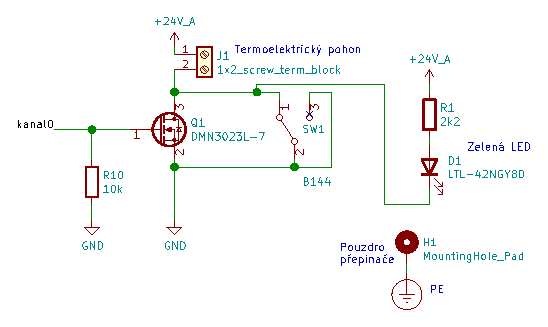
\includegraphics[width=\textwidth]{images/svg/kicad/zonovy-regulator-mosfet-pwm-1-kanal.eps}
    \caption{Zapojení jednoho kanálu pro ovládání termoelektrického pohonu.}
    \label{fig:zonovy-regulator-mosfet-pwm-1-kanal}
\end{figure}

\begin{figure}[H]
    \centering
    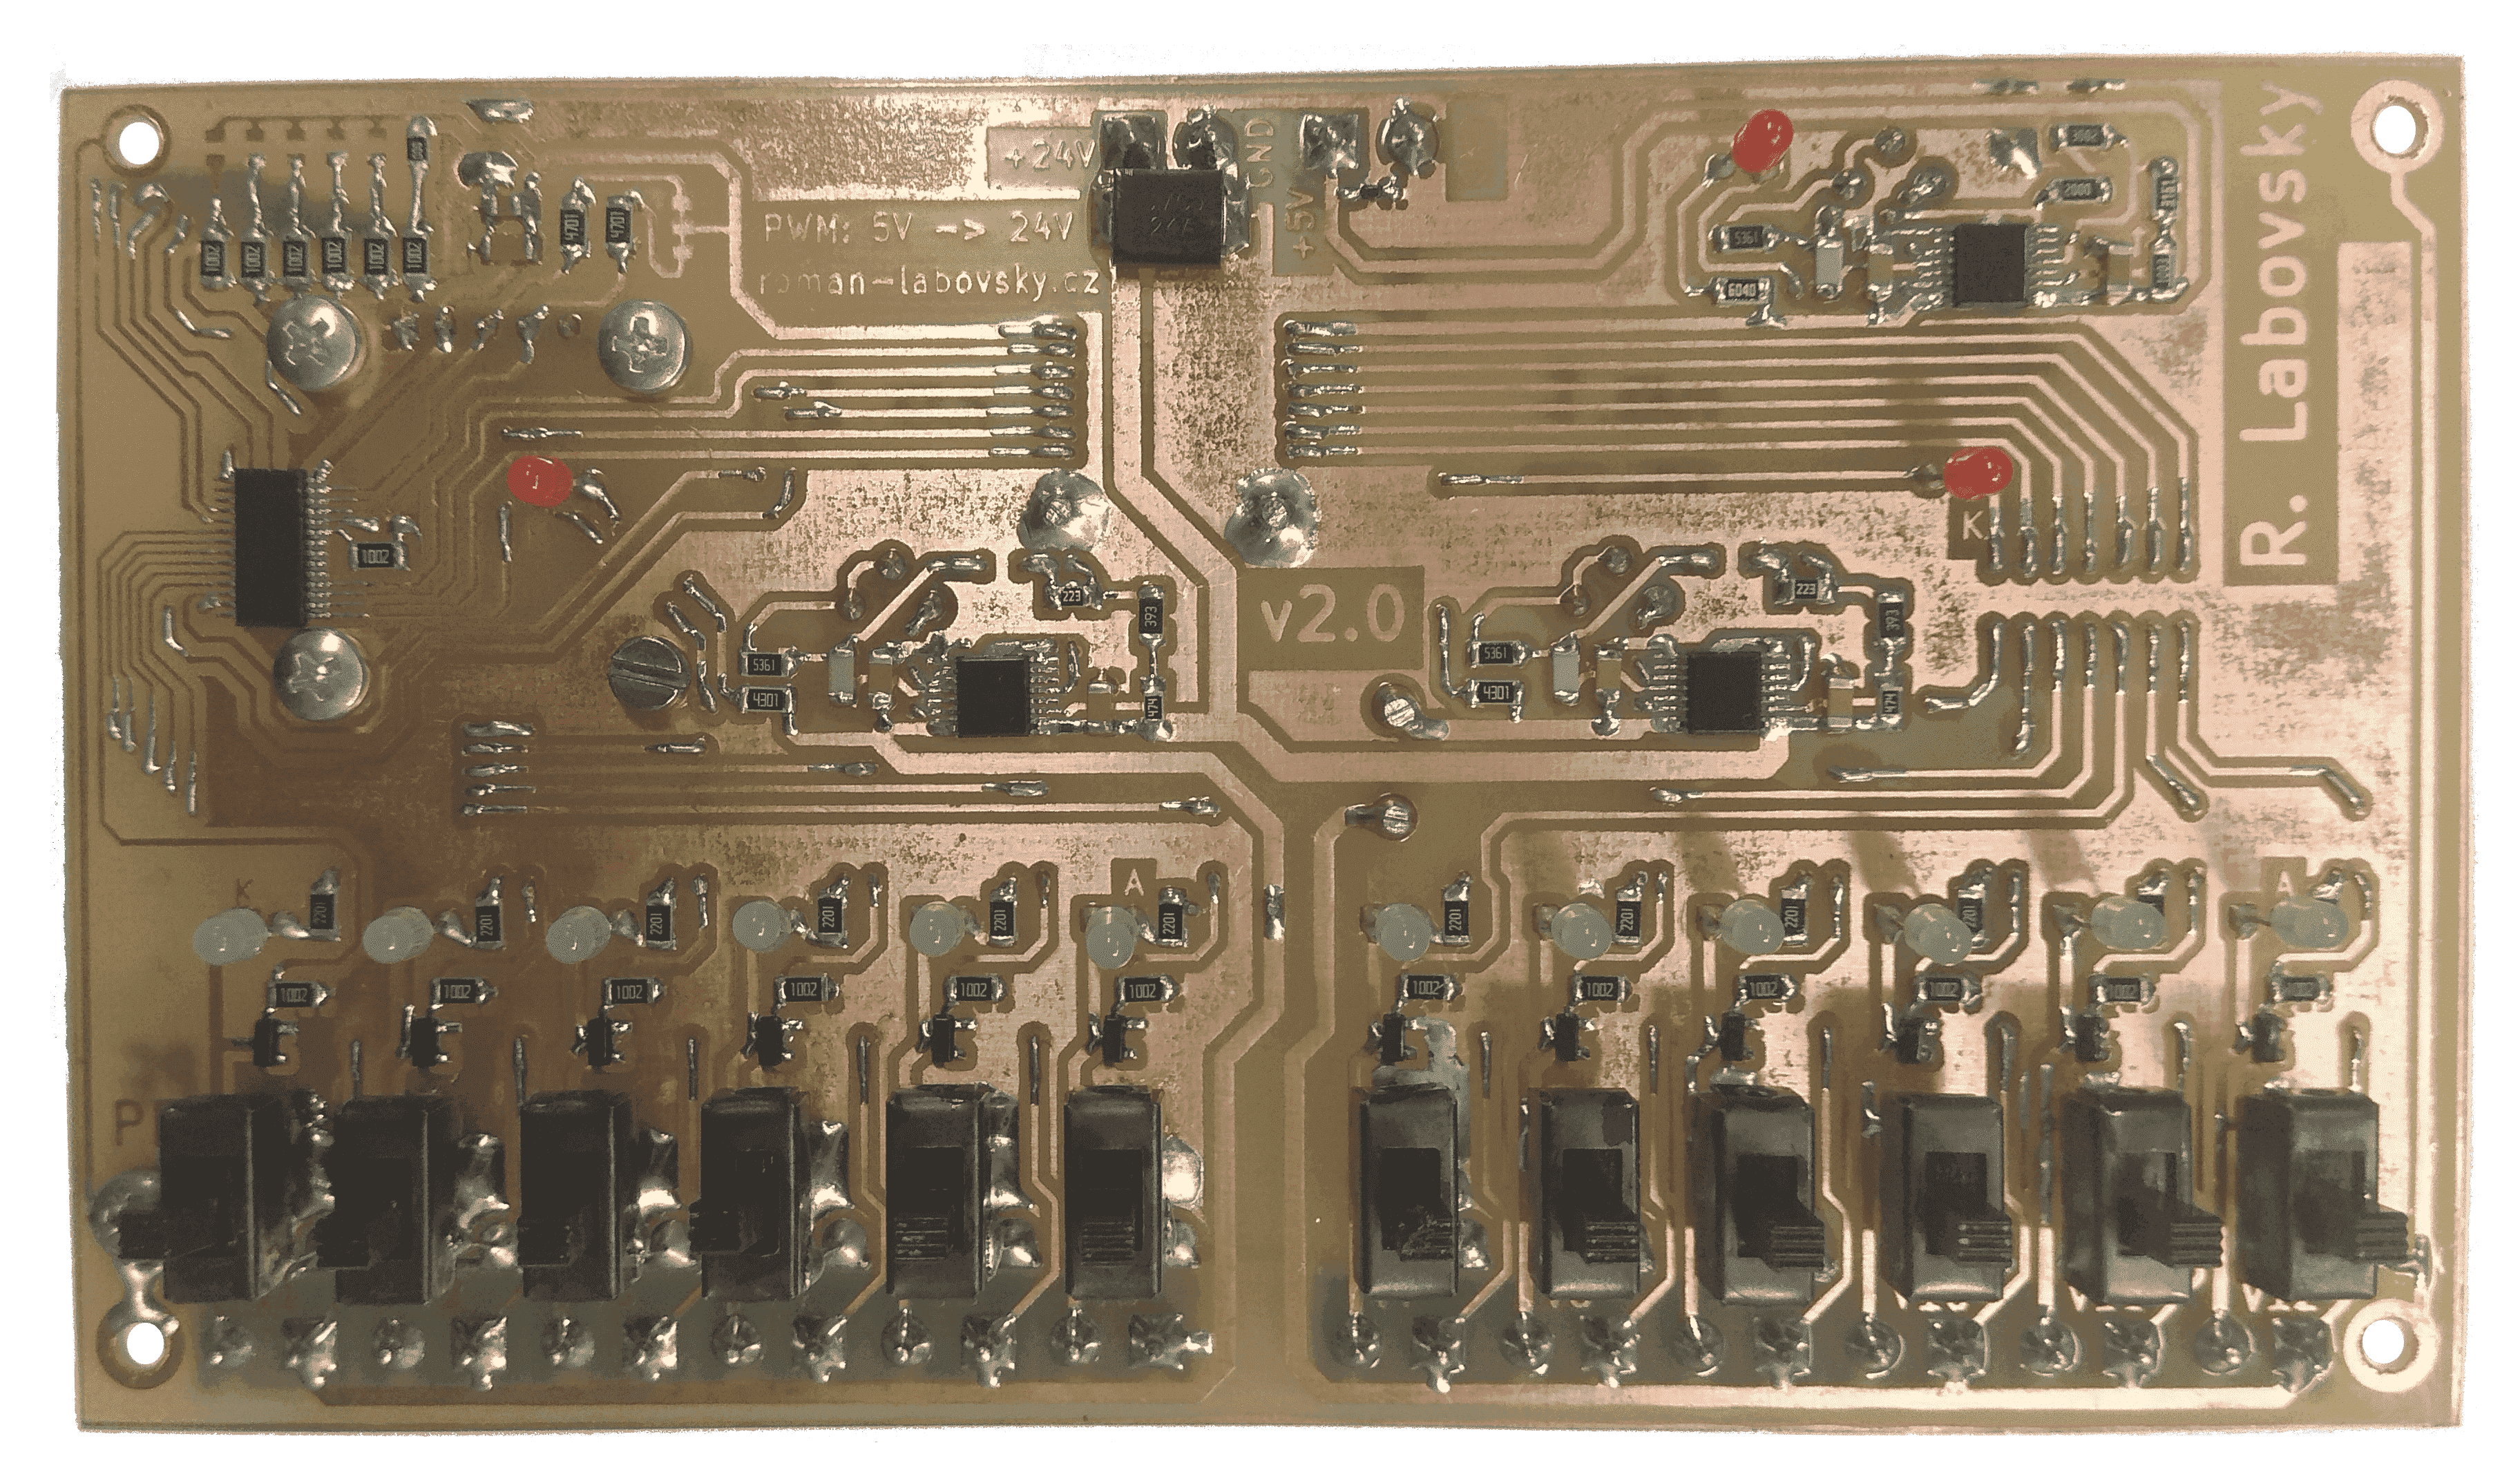
\includegraphics[width=0.99\textwidth]{images/zonovy-regulator/dps-zonovy-regulator-spodni-strana.png}
    \caption{DPS zónového regulátoru, spodní strana.}
    \label{fig:dps-zonovy-regulator-spodni-strana}
\end{figure}

\begin{figure}[H]
    \centering
    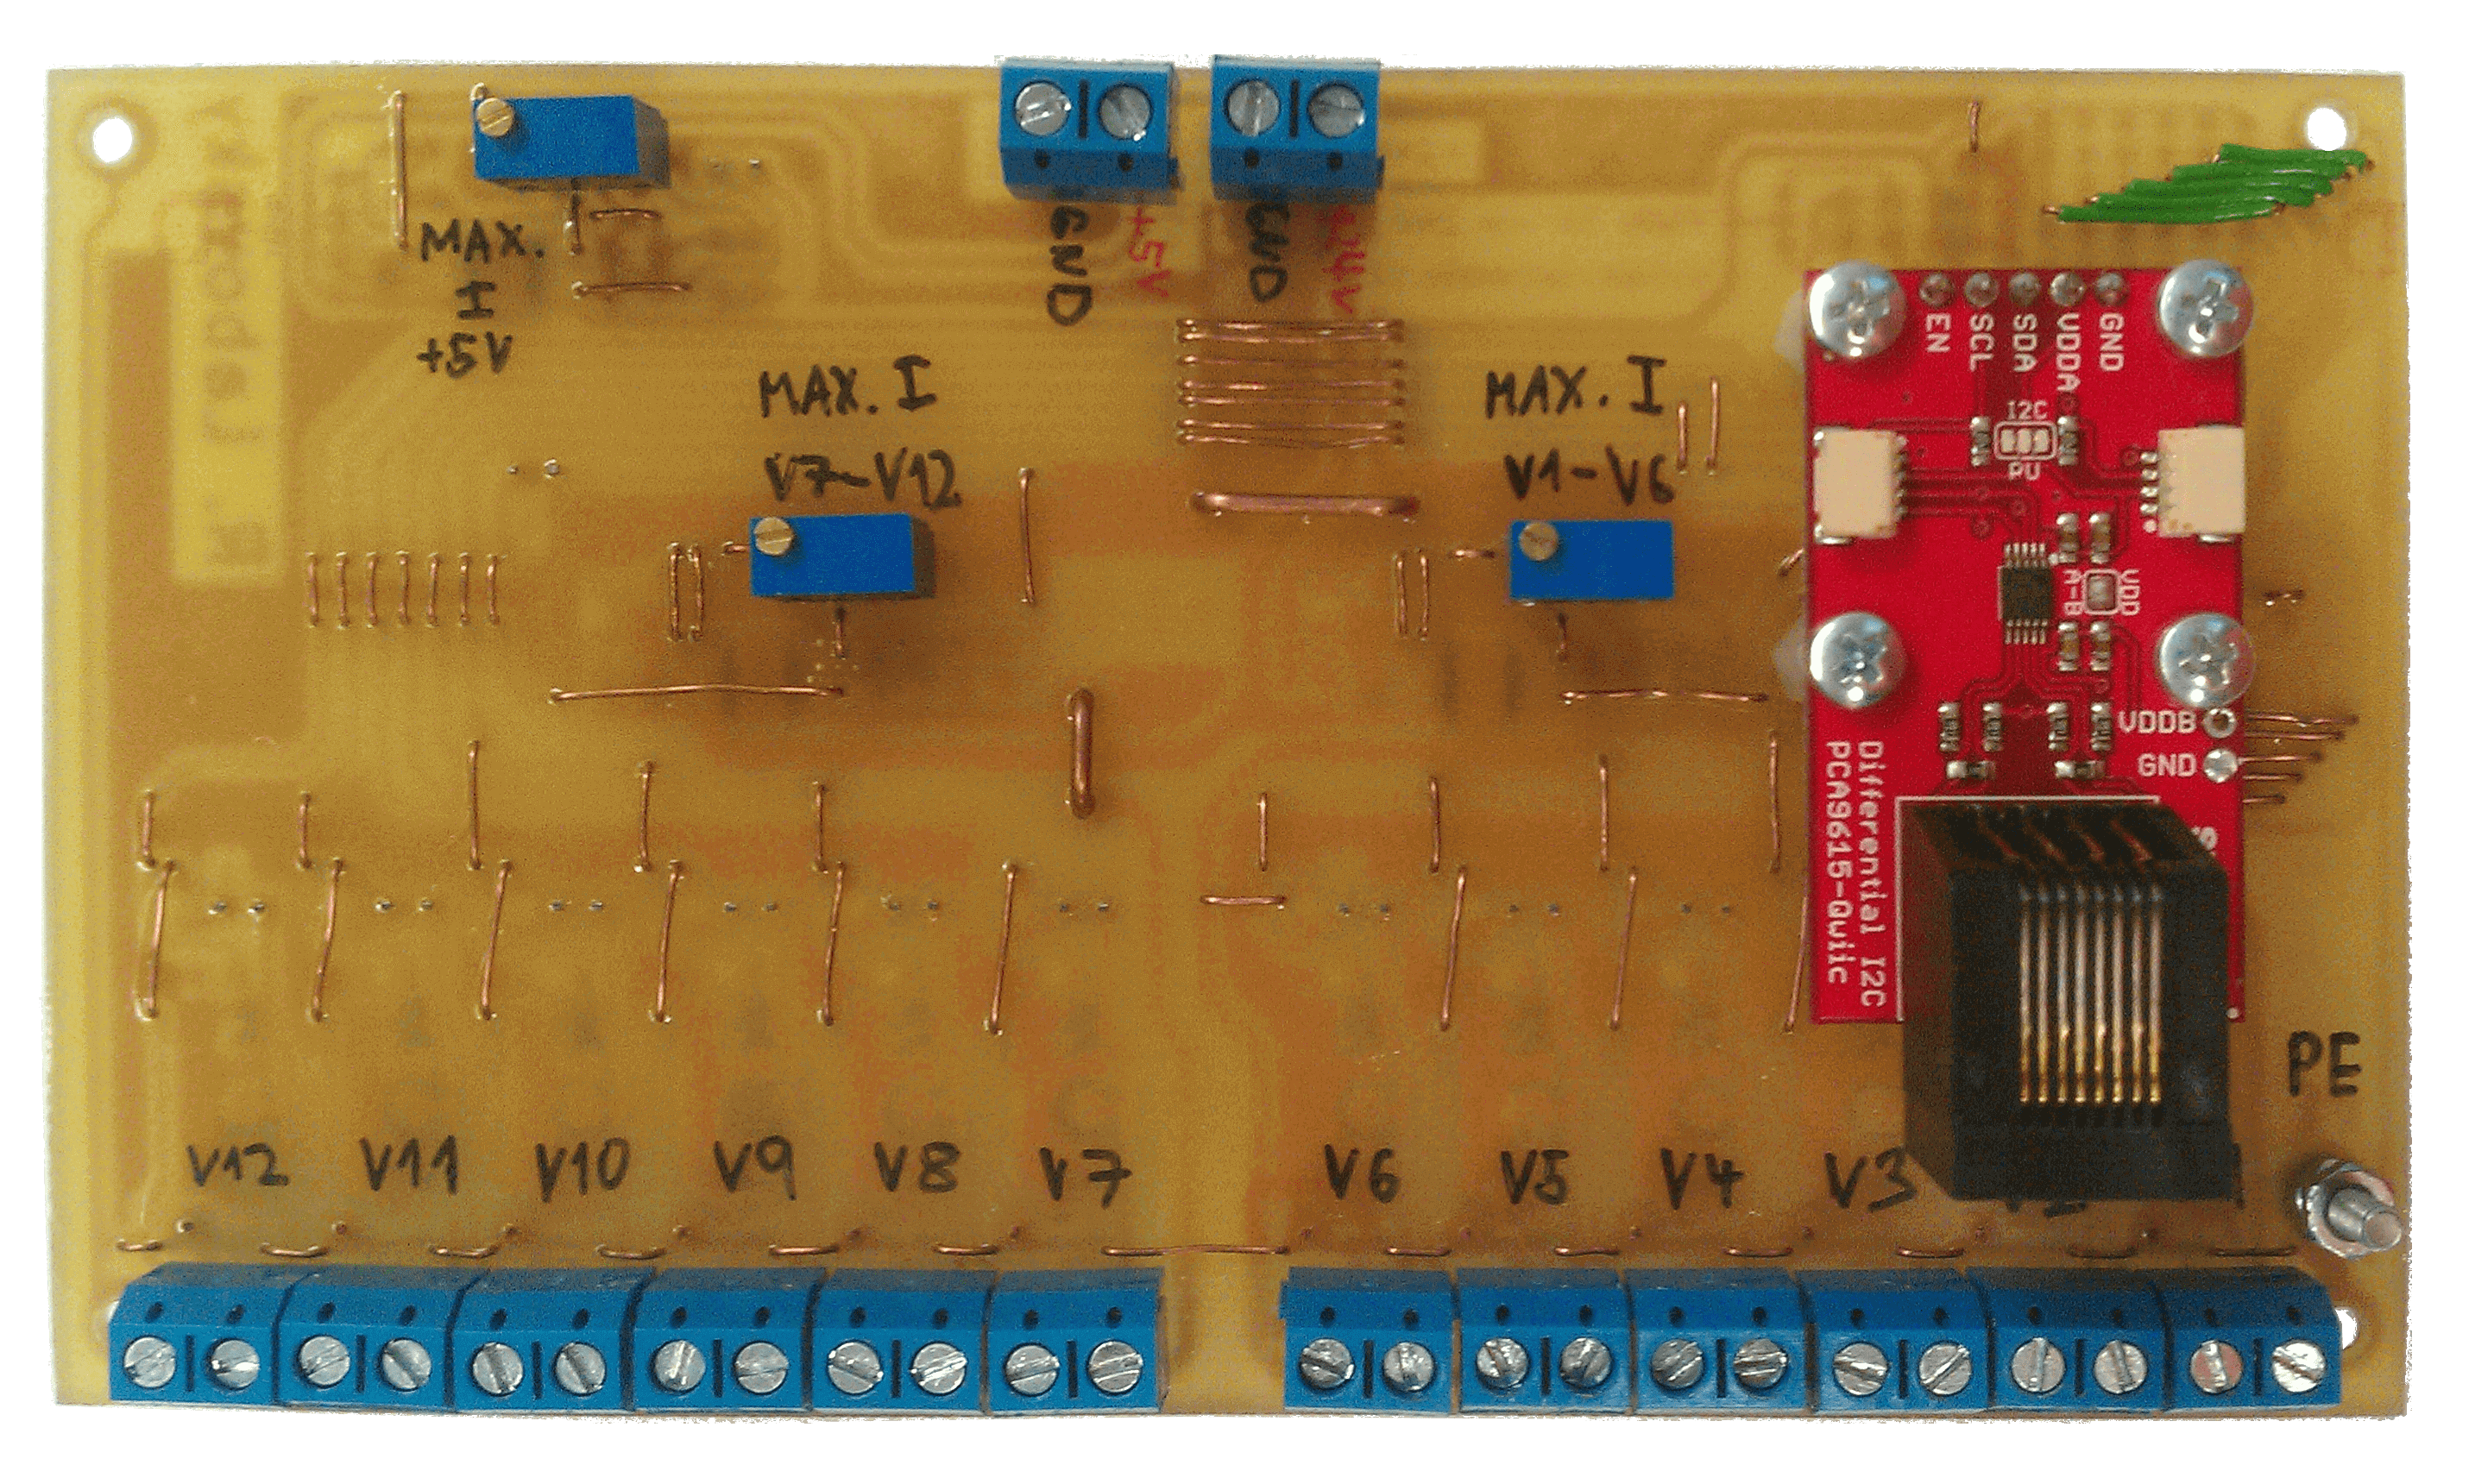
\includegraphics[width=0.99\textwidth]{images/zonovy-regulator/dps-zonovy-regulator-vrchni-strana.png}
    \caption{DPS zónového regulátoru, vrchní strana.}
    \label{fig:dps-zonovy-regulator-vrchni-strana}
\end{figure}


\begin{figure}[H]
    \centering
    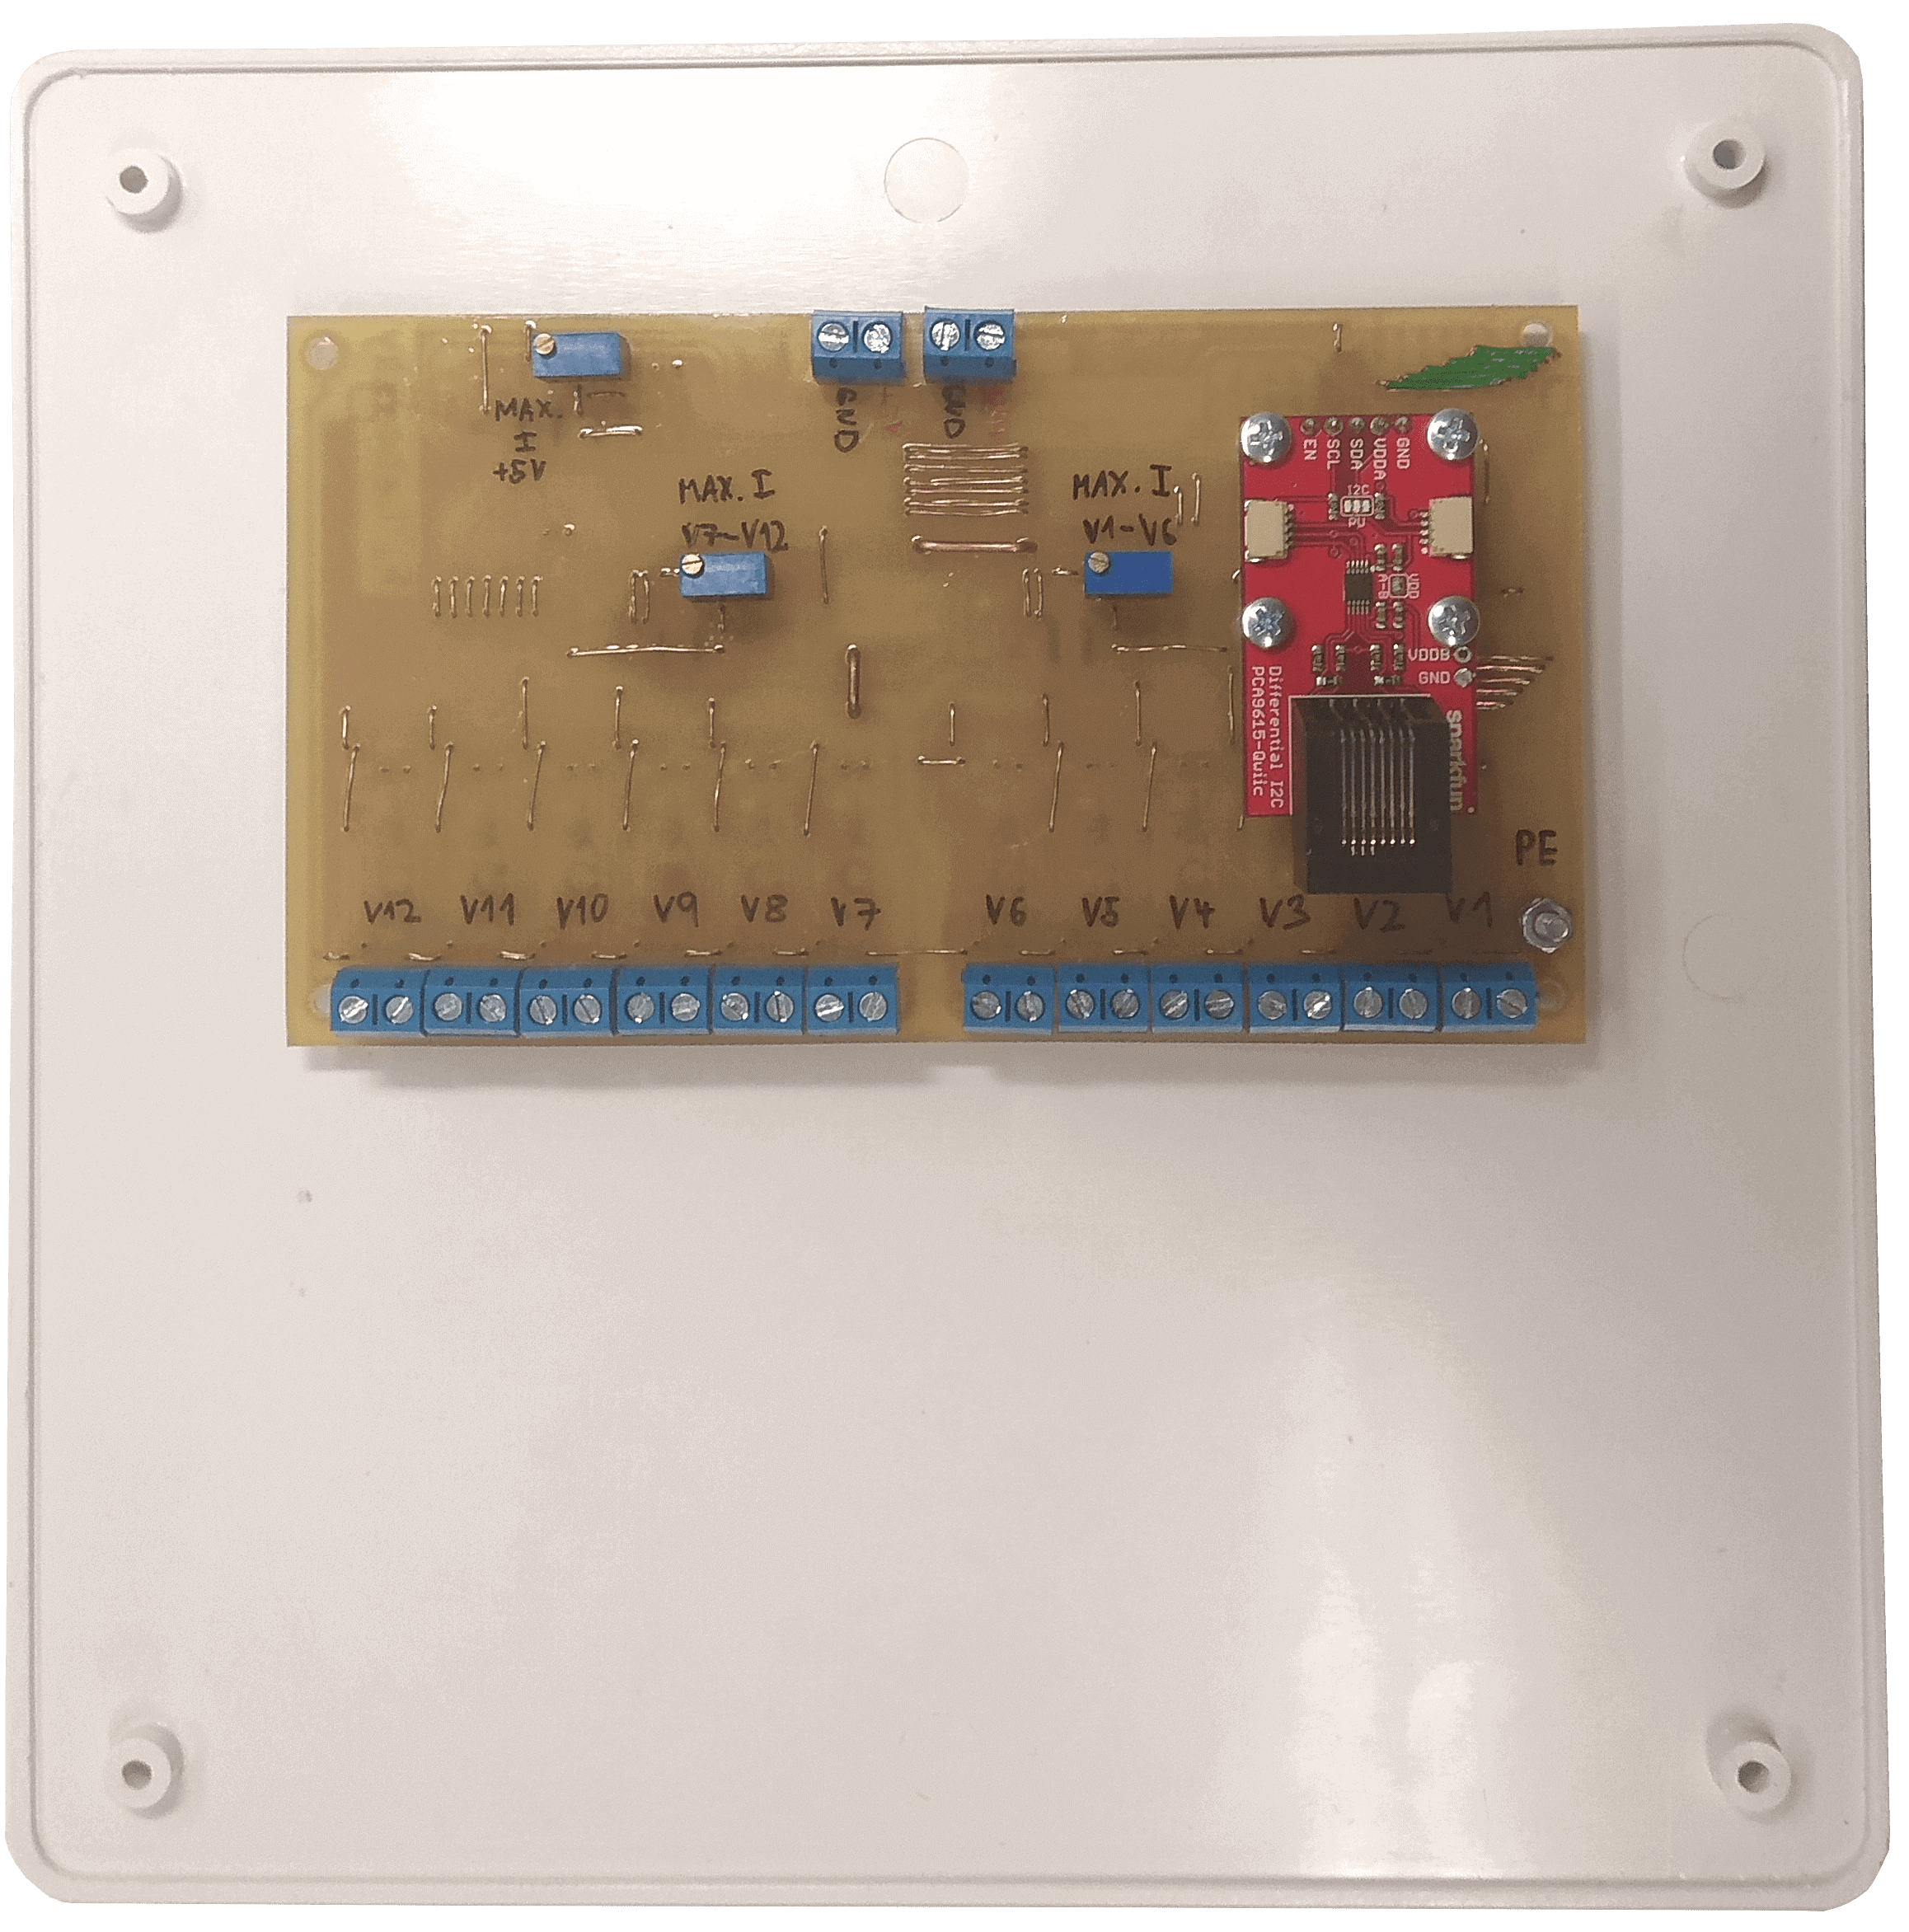
\includegraphics[width=0.95\textwidth]{images/zonovy-regulator/zonovy-regulator-spodni-strana.png}
    \caption{Zadní část panelu zónového regulátoru.}
    \label{fig:zonovy-regulator-spodni-strana}
\end{figure}

\begin{figure}[H]
    \centering
    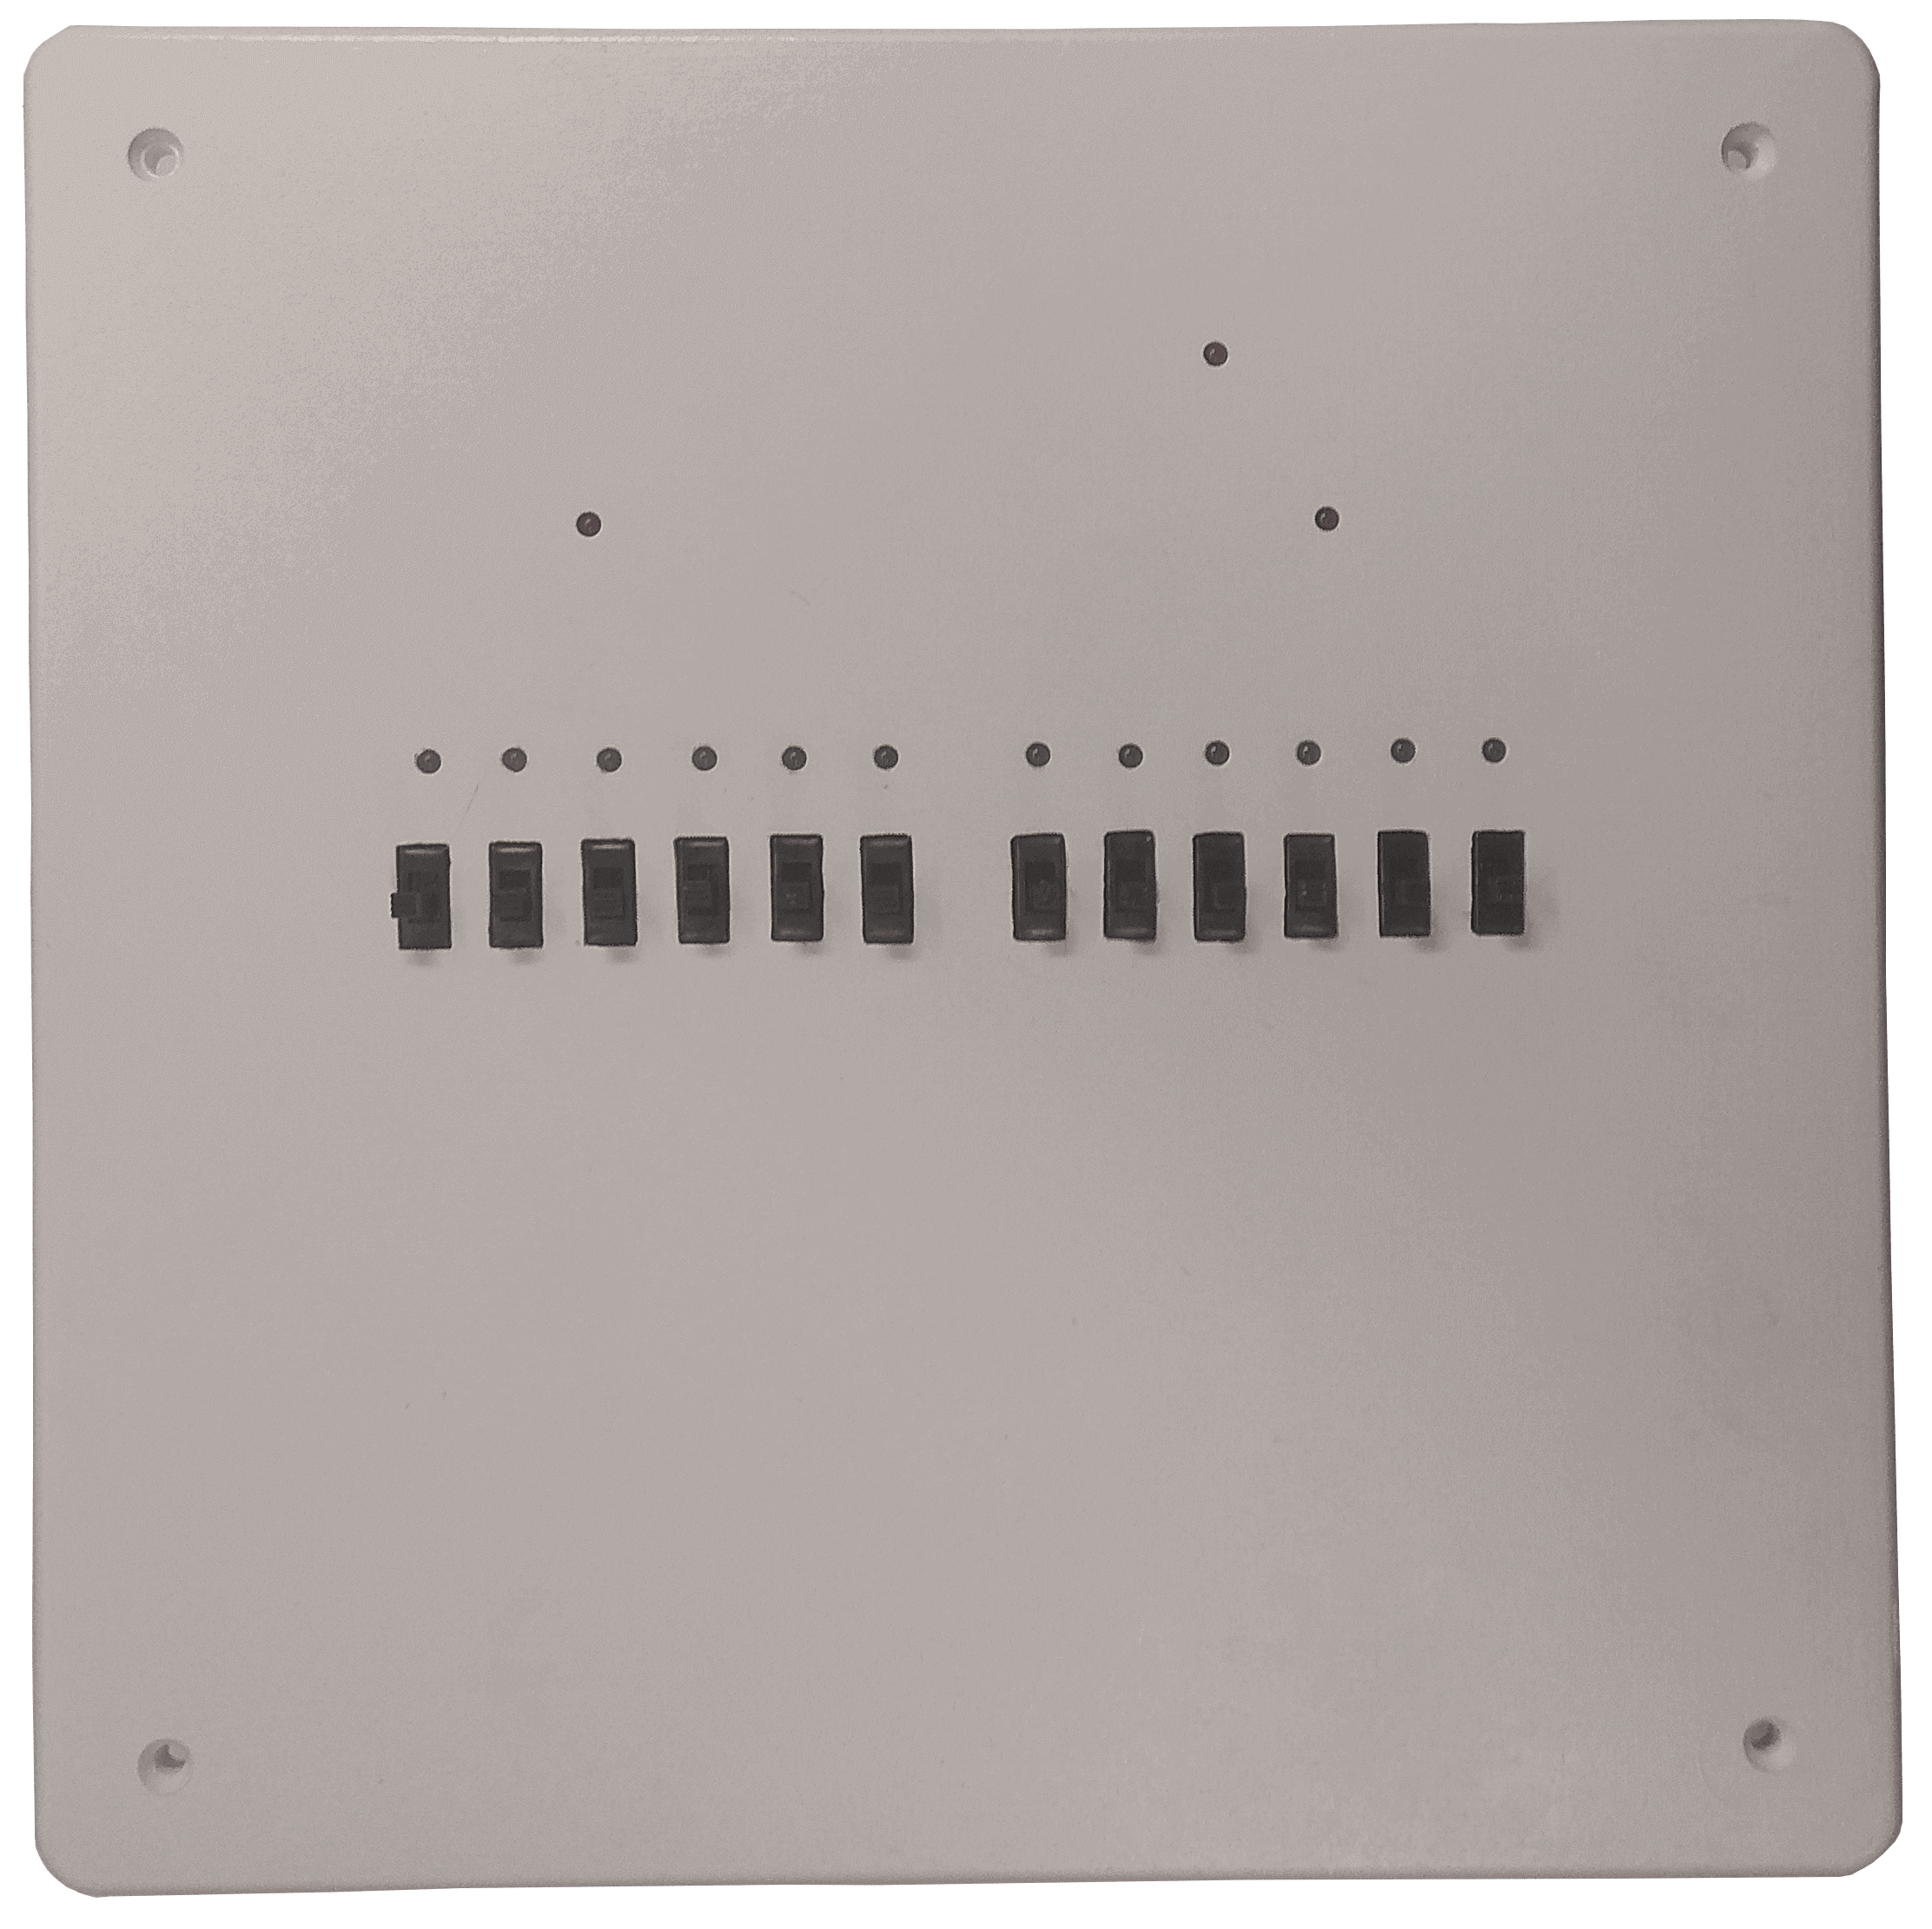
\includegraphics[width=0.95\textwidth]{images/zonovy-regulator/zonovy-regulator-vrchni-strana.png}
    \caption[Čelní část panelu zónového regulátoru.]{Čelní část panelu zónového regulátoru se signalizačními LED a~manuálním ovládáním pomocí spínačů.}
    \label{fig:zonovy-regulator-vrchni-strana}
\end{figure}



\subsubsection{Termoelektrické pohony Salus T30NC}  
Termoelektrický pohon Salus T30NC slouží k ovládání ventilů pro jednotlivé otopné okruhy. Je napájen stejnosměrným napětí 24 V při maximálním proudovém odběru při zapnutí 250 mA. Provozní příkon jsou 2 W. Rozměr závitu je M30\,×\,1,5. Maximální délka zdvihu pro dřík ventilu činí 4 mm. Síla pohonu je 100 N ($\pm$10 \%). Čas pro otevření je přibližně 2 minuty. Jedná se o~typ \acrshort{nc} (\textit{\acrlong{nc}}). Při odpojení napájení je ventil zavřen. Pohon má funkci „First Open“, neboli je možné pomocí zarážky ventil instalovat jako otevřený bez nutnosti napájení (využít v případě, kdy není ještě instalovaná centrální jednotka). Pro každé patro je použito 12 těchto pohonů.

\begin{figure}[H]
    \centering
    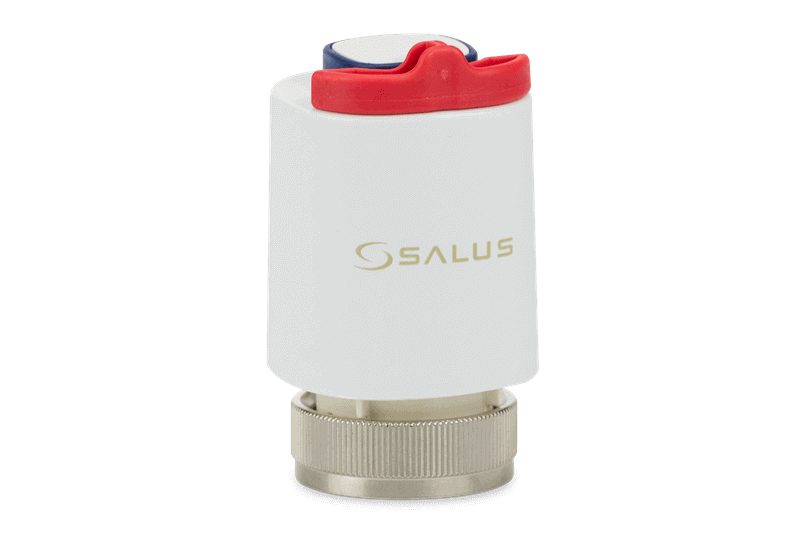
\includegraphics[width=0.8\textwidth]{images/termoelektricky-pohon-salus-t30nc-24-v.png}
    \caption[Termoelektrický pohon Salus T30NC.]{Termoelektrický pohon Salus T30NC na stejnosměrné napětí 24~V \cite{termoelektricky-pohon-t30nc}.}
    \label{fig:termoelektricky-pohon-salus-t30nc-24-v}
\end{figure}